
\documentclass[10pt, conference,compsoc]{IEEEtran}
\usepackage{hyperref}
\usepackage{graphicx}
\usepackage{cite}
\usepackage[T1]{fontenc}
\usepackage[utf8]{inputenc}
\usepackage{parselines} 
\usepackage{listings}
\usepackage{float}
% Some/most Computer Society conferences require the compsoc mode option,
% but others may want the standard conference format.
%
% If IEEEtran.cls has not been installed into the LaTeX system files,
% manually specify the path to it like:
% \documentclass[conference,compsoc]{../sty/IEEEtran}





% Some very useful LaTeX packages include:
% (uncomment the ones you want to load)


% *** MISC UTILITY PACKAGES ***
%
%\usepackage{ifpdf}
% Heiko Oberdiek's ifpdf.sty is very useful if you need conditional
% compilation based on whether the output is pdf or dvi.
% usage:
% \ifpdf
%   % pdf code
% \else
%   % dvi code
% \fi
% The latest version of ifpdf.sty can be obtained from:
% http://www.ctan.org/pkg/ifpdf
% Also, note that IEEEtran.cls V1.7 and later provides a builtin
% \ifCLASSINFOpdf conditional that works the same way.
% When switching from latex to pdflatex and vice-versa, the compiler may
% have to be run twice to clear warning/error messages.






% *** CITATION PACKAGES ***
%
\ifCLASSOPTIONcompsoc
  % IEEE Computer Society needs nocompress option
  % requires cite.sty v4.0 or later (November 2003)
  \usepackage{amsmath}
\else
  % normal IEEE
  \usepackage{cite}
\fi
% cite.sty was written by Donald Arseneau
% V1.6 and later of IEEEtran pre-defines the format of the cite.sty package
% \cite{} output to follow that of the IEEE. Loading the cite package will
% result in citation numbers being automatically sorted and properly
% "compressed/ranged". e.g., [1], [9], [2], [7], [5], [6] without using
% cite.sty will become [1], [2], [5]--[7], [9] using cite.sty. cite.sty's
% \cite will automatically add leading space, if needed. Use cite.sty's
% noadjust option (cite.sty V3.8 and later) if you want to turn this off
% such as if a citation ever needs to be enclosed in parenthesis.
% cite.sty is already installed on most LaTeX systems. Be sure and use
% version 5.0 (2009-03-20) and later if using hyperref.sty.
% The latest version can be obtained at:
% http://www.ctan.org/pkg/cite
% The documentation is contained in the cite.sty file itself.
%
% Note that some packages require special options to format as the Computer
% Society requires. In particular, Computer Society  papers do not use
% compressed citation ranges as is done in typical IEEE papers
% (e.g., [1]-[4]). Instead, they list every citation separately in order
% (e.g., [1], [2], [3], [4]). To get the latter we need to load the cite
% package with the nocompress option which is supported by cite.sty v4.0
% and later.





% *** GRAPHICS RELATED PACKAGES ***
%
\ifCLASSINFOpdf
  % \usepackage[pdftex]{graphicx}
  % declare the path(s) where your graphic files are
  % \graphicspath{{../pdf/}{../jpeg/}}
  % and their extensions so you won't have to specify these with
  % every instance of \includegraphics
  % \DeclareGraphicsExtensions{.pdf,.jpeg,.png}
\else
  % or other class option (dvipsone, dvipdf, if not using dvips). graphicx
  % will default to the driver specified in the system graphics.cfg if no
  % driver is specified.
  % \usepackage[dvips]{graphicx}
  % declare the path(s) where your graphic files are
  % \graphicspath{{../eps/}}
  % and their extensions so you won't have to specify these with
  % every instance of \includegraphics
  % \DeclareGraphicsExtensions{.eps}
\fi
% graphicx was written by David Carlisle and Sebastian Rahtz. It is
% required if you want graphics, photos, etc. graphicx.sty is already
% installed on most LaTeX systems. The latest version and documentation
% can be obtained at: 
% http://www.ctan.org/pkg/graphicx
% Another good source of documentation is "Using Imported Graphics in
% LaTeX2e" by Keith Reckdahl which can be found at:
% http://www.ctan.org/pkg/epslatex
%
% latex, and pdflatex in dvi mode, support graphics in encapsulated
% postscript (.eps) format. pdflatex in pdf mode supports graphics
% in .pdf, .jpeg, .png and .mps (metapost) formats. Users should ensure
% that all non-photo figures use a vector format (.eps, .pdf, .mps) and
% not a bitmapped formats (.jpeg, .png). The IEEE frowns on bitmapped formats
% which can result in "jaggedy"/blurry rendering of lines and letters as
% well as large increases in file sizes.
%
% You can find documentation about the pdfTeX application at:
% http://www.tug.org/applications/pdftex





% *** MATH PACKAGES ***
%
%\usepackage{amsmath}
% A popular package from the American Mathematical Society that provides
% many useful and powerful commands for dealing with mathematics.
%
% Note that the amsmath package sets \interdisplaylinepenalty to 10000
% thus preventing page breaks from occurring within multiline equations. Use:
%\interdisplaylinepenalty=2500
% after loading amsmath to restore such page breaks as IEEEtran.cls normally
% does. amsmath.sty is already installed on most LaTeX systems. The latest
% version and documentation can be obtained at:
% http://www.ctan.org/pkg/amsmath





% *** SPECIALIZED LIST PACKAGES ***
%
%\usepackage{algorithmic}
% algorithmic.sty was written by Peter Williams and Rogerio Brito.
% This package provides an algorithmic environment fo describing algorithms.
% You can use the algorithmic environment in-text or within a figure
% environment to provide for a floating algorithm. Do NOT use the algorithm
% floating environment provided by algorithm.sty (by the same authors) or
% algorithm2e.sty (by Christophe Fiorio) as the IEEE does not use dedicated
% algorithm float types and packages that provide these will not provide
% correct IEEE style captions. The latest version and documentation of
% algorithmic.sty can be obtained at:
% http://www.ctan.org/pkg/algorithms
% Also of interest may be the (relatively newer and more customizable)
% algorithmicx.sty package by Szasz Janos:
% http://www.ctan.org/pkg/algorithmicx




% *** ALIGNMENT PACKAGES ***
%
%\usepackage{array}
% Frank Mittelbach's and David Carlisle's array.sty patches and improves
% the standard LaTeX2e array and tabular environments to provide better
% appearance and additional user controls. As the default LaTeX2e table
% generation code is lacking to the point of almost being broken with
% respect to the quality of the end results, all users are strongly
% advised to use an enhanced (at the very least that provided by array.sty)
% set of table tools. array.sty is already installed on most systems. The
% latest version and documentation can be obtained at:
% http://www.ctan.org/pkg/array


% IEEEtran contains the IEEEeqnarray family of commands that can be used to
% generate multiline equations as well as matrices, tables, etc., of high
% quality.




% *** SUBFIGURE PACKAGES ***
%\ifCLASSOPTIONcompsoc
%  \usepackage[caption=false,font=footnotesize,labelfont=sf,textfont=sf]{subfig}
%\else
%  \usepackage[caption=false,font=footnotesize]{subfig}
%\fi
% subfig.sty, written by Steven Douglas Cochran, is the modern replacement
% for subfigure.sty, the latter of which is no longer maintained and is
% incompatible with some LaTeX packages including fixltx2e. However,
% subfig.sty requires and automatically loads Axel Sommerfeldt's caption.sty
% which will override IEEEtran.cls' handling of captions and this will result
% in non-IEEE style figure/table captions. To prevent this problem, be sure
% and invoke subfig.sty's "caption=false" package option (available since
% subfig.sty version 1.3, 2005/06/28) as this is will preserve IEEEtran.cls
% handling of captions.
% Note that the Computer Society format requires a sans serif font rather
% than the serif font used in traditional IEEE formatting and thus the need
% to invoke different subfig.sty package options depending on whether
% compsoc mode has been enabled.
%
% The latest version and documentation of subfig.sty can be obtained at:
% http://www.ctan.org/pkg/subfig




% *** FLOAT PACKAGES ***
%
%\usepackage{fixltx2e}
% fixltx2e, the successor to the earlier fix2col.sty, was written by
% Frank Mittelbach and David Carlisle. This package corrects a few problems
% in the LaTeX2e kernel, the most notable of which is that in current
% LaTeX2e releases, the ordering of single and double column floats is not
% guaranteed to be preserved. Thus, an unpatched LaTeX2e can allow a
% single column figure to be placed prior to an earlier double column
% figure.
% Be aware that LaTeX2e kernels dated 2015 and later have fixltx2e.sty's
% corrections already built into the system in which case a warning will
% be issued if an attempt is made to load fixltx2e.sty as it is no longer
% needed.
% The latest version and documentation can be found at:
% http://www.ctan.org/pkg/fixltx2e


%\usepackage{stfloats}
% stfloats.sty was written by Sigitas Tolusis. This package gives LaTeX2e
% the ability to do double column floats at the bottom of the page as well
% as the top. (e.g., "\begin{figure*}[!b]" is not normally possible in
% LaTeX2e). It also provides a command:
%\fnbelowfloat
% to enable the placement of footnotes below bottom floats (the standard
% LaTeX2e kernel puts them above bottom floats). This is an invasive package
% which rewrites many portions of the LaTeX2e float routines. It may not work
% with other packages that modify the LaTeX2e float routines. The latest
% version and documentation can be obtained at:
% http://www.ctan.org/pkg/stfloats
% Do not use the stfloats baselinefloat ability as the IEEE does not allow
% \baselineskip to stretch. Authors submitting work to the IEEE should note
% that the IEEE rarely uses double column equations and that authors should try
% to avoid such use. Do not be tempted to use the cuted.sty or midfloat.sty
% packages (also by Sigitas Tolusis) as the IEEE does not format its papers in
% such ways.
% Do not attempt to use stfloats with fixltx2e as they are incompatible.
% Instead, use Morten Hogholm'a dblfloatfix which combines the features
% of both fixltx2e and stfloats:
%
% \usepackage{dblfloatfix}
% The latest version can be found at:
% http://www.ctan.org/pkg/dblfloatfix




% *** PDF, URL AND HYPERLINK PACKAGES ***
%
%\usepackage{url}
% url.sty was written by Donald Arseneau. It provides better support for
% handling and breaking URLs. url.sty is already installed on most LaTeX
% systems. The latest version and documentation can be obtained at:
% http://www.ctan.org/pkg/url
% Basically, \url{my_url_here}.




% *** Do not adjust lengths that control margins, column widths, etc. ***
% *** Do not use packages that alter fonts (such as pslatex).         ***
% There should be no need to do such things with IEEEtran.cls V1.6 and later.
% (Unless specifically asked to do so by the journal or conference you plan
% to submit to, of course. )


% correct bad hyphenation here
\hyphenation{op-tical net-works semi-conduc-tor}


\begin{document}
%
% paper title
% Titles are generally capitalized except for words such as a, an, and, as,
% at, but, by, for, in, nor, of, on, or, the, to and up, which are usually
% not capitalized unless they are the first or last word of the title.
% Linebreaks \\ can be used within to get better formatting as desired.
% Do not put math or special symbols in the title.
\title{Aridac: Adaptive Resource Isolation of Non-volatile Devices \\Under  Containerized Environment \\ Project Final Report}


% author names and affiliations
% use a multiple column layout for up to three different
% affiliations
\author{
\IEEEauthorblockN{Xiang Yue}
\IEEEauthorblockA{School of Computer Science\\
Carnegie Mellon University\\
Pittsburgh, Pennsylvania 15213\\
Email: xiangyue@andrew.cmu.edu}
\and
\IEEEauthorblockN{Xuan Peng}
\IEEEauthorblockA{Information Networking Institute\\
Carnegie Mellon University\\
Pittsburgh, Pennsylvania 15213\\
Email: xuanpeng@andrew.cmu.edu}
\and
\IEEEauthorblockN{Zeyu Wang}
\IEEEauthorblockA{Information Networking Institute\\
Carnegie Mellon University\\
Pittsburgh, Pennsylvania 15213\\
Email: zeyuwang@cmu.edu}
}


% conference papers do not typically use \thanks and this command
% is locked out in conference mode. If really needed, such as for
% the acknowledgment of grants, issue a \IEEEoverridecommandlockouts
% after \documentclass

% for over three affiliations, or if they all won't fit within the width
% of the page (and note that there is less available width in this regard for
% compsoc conferences compared to traditional conferences), use this
% alternative format:
% 
%\author{\IEEEauthorblockN{Michael Shell\IEEEauthorrefmark{1},
%Homer Simpson\IEEEauthorrefmark{2},
%James Kirk\IEEEauthorrefmark{3}, 
%Montgomery Scott\IEEEauthorrefmark{3} and
%Eldon Tyrell\IEEEauthorrefmark{4}}
%\IEEEauthorblockA{\IEEEauthorrefmark{1}School of Electrical and Computer Engineering\\
%Georgia Institute of Technology,
%Atlanta, Georgia 30332--0250\\ Email: see http://www.michaelshell.org/contact.html}
%\IEEEauthorblockA{\IEEEauthorrefmark{2}Twentieth Century Fox, Springfield, USA\\
%Email: homer@thesimpsons.com}
%\IEEEauthorblockA{\IEEEauthorrefmark{3}Starfleet Academy, San Francisco, California 96678-2391\\
%Telephone: (800) 555--1212, Fax: (888) 555--1212}
%\IEEEauthorblockA{\IEEEauthorrefmark{4}Tyrell Inc., 123 Replicant Street, Los Angeles, California 90210--4321}}




% use for special paper notices
%\IEEEspecialpapernotice{(Invited Paper)}




% make the title area
\maketitle

% As a general rule, do not put math, special symbols or citations
% in the abstract
\begin{abstract}
Container technology makes cloud computing possible by offering resource isolation and scalability, however, resource sharing brings the problem where heavy containers consume most of the resources and break the fairness. To achieve fairness and maintain a good overall system performance, we propose an adaptive resource isolator for block device namely Aridac, which could adjust the disk resource quota of containers in running time.
\end{abstract}

% no keywords




% For peer review papers, you can put extra information on the cover
% page as needed:
% \ifCLASSOPTIONpeerreview
% \begin{center} \bfseries EDICS Category: 3-BBND \end{center}
% \fi
%
% For peerreview papers, this IEEEtran command inserts a page break and
% creates the second title. It will be ignored for other modes.
\IEEEpeerreviewmaketitle



\section{Introduction}
Cloud computing platforms, as a typical instance of infrastructure-as-a-service, nowadays have become the first choice for internet application developers to deploy their services. The main reason behind the popularity is - cloud computing offers reliability, convenience, isolation, and scalability, along with the pay-as-you-go pricing model. To achieve those features, the quality of service must be ensured with the achievement of resources isolation technologies.\\

Container, as the core part of isolation, creates an illusion for customers as owning the entire system. This lightweight virtualization notion has been widely leveraged by cloud service providers. Based on Linux Cgroup, which offers the ability to isolate resource (e.g. namespace, network I/O, disk I/O), container technologies and applications raised, like Linux Container (LXC) \cite{lxc} and Docker \cite{docker}. Those form the basic units of cloud platforms and are still a great domain for cloud providers to dive deep into. \\

However, behind the great idea of containerization, there come new problems with resources isolation in practice. One of the glaring issues to resolve is resource allocation fairness, which means avoiding the resources allocated to containers interfering with each other. For instance, when there are several containers within a node and one of them is running heavy workloads with intense I/O operations, the resources of other nodes can be consumed, greatly delaying the delivery of tasks, like the completion of file reading, the transmission of RPC requests, etc. In addition, Xavier et al. \cite{Xavier2015API} has also analyzed and confirmed the interference of heavy disk workload without limits on resource allocation can degrade the overall performance of the system. Therefore, to avoid sudden delay of container processes, a limitation of resource quota is a good way to control.\\

Although there are already some tools (cgroup, trickle) for adjusting resource quota, the problem is, those tools only offer fixed limitations of resource quota, whereas, in industry, cloud providers can never know how to adjust quota in advance or in real-time - the application in containers and containers themselves are dynamically created, killed and changed frequently. In addition, one of our group members met with the same problem with an intolerant latency of services when resources are consumed mostly by a disk-intensive container. Some works \cite{Sungyong16} manages to alleviate the issue. Since there are still few efforts working on this topic in both academy and industry, our group planned to look into a dynamic way of isolation adjustment.\\

We plan to propose the Aridac, an Adaptive Resource Isolation algorithm of Non-volatile Devices under heterogeneous containerized environment. The basic idea is to monitor, collect and analyze the resource usage habit of containers as time goes on, and allocate their resources to ensure fairness under certain rules. The quota of disk I/O can be allocated by, for instance, the priority of the application, or by containers' history maximum usage. And the objective is to achieve fairness. Besides the algorithm, we plan to design the testing workloads and design experiments for comparing fairness between different policies with specific metrics. Also, we will provide the corresponding benchmark data for further research. To narrow down the scope, we focus on disk isolation, which can be extended to the network I/O or other resources allocation scenario. The basic tools of system design and experiments include cgroup, bash scripts.\\

The rest of the proposal is organized as follows: Related Work section shows the relevant works of disk I/O isolation; Methodology section shows how we will define the effectiveness of Aridac; Goals includes our promising results of research; Final paper plan illustrates how we will write the final paper. 

\section{Related Works}
Currently, there are not so many efforts on research of container isolation, especially on disk I/O. However, some researchers interested in disk I/O isolation has some works for us to refer. Merchant et al. \cite{Merchant2011MaestroQI} proposed Maestro, focused on the fairness and performance of disk I/O allocation for different applications. He hypothesized there are different performance targets (throughput or I/O directed) for each application, and developed a policy to allocate the resources to them to reach the best overall performance. Arunagiri et al.\cite{Arunagiri2011FAIRIOAA} developed the FAIRIO algorithm to schedule prorated I/O resources for fair allocation, which is a more general solution. Li et al.\cite{Li2015ASCARAC} provided an automatic framework to monitor storage contention and optimize bandwidth utilization. In addtion, for the different scenario on solid state disks, Jo et al.\cite{Jo2017DynamicLB} proposed a I/O load balancer for it. \\

The above ideas give us a good inspiration for container disk I/O isolation. However, those works are not strongly related to our topic. Take Maestro as an instance, it focuses on application I/O balancing on large disk arrays, so its algorithm takes disk I/O ports and preset application targats in consideration with optimization function, which is not aligned with our topic.\\

A naive idea is to treat containers as applications and apply the above solutions. However, different from applications, containers' behaviors are more complicated. In this paper, we believe each container has a dynamic usage pattern and is variable from period to period. Therefore, adjusting the policy to allocate resources cannot be avoided.\\

As for resource isolation tools, Linux control group (cgroup) is the original resource isolation tools, and docker's isolation capacity is built on this. We can easily find the corresonding cgroup of each docker container to limit there resource usage.\\


% An example of a floating figure using the graphicx package.
% Note that \label must occur AFTER (or within) \caption.
% For figures, \caption should occur after the \includegraphics.
% Note that IEEEtran v1.7 and later has special internal code that
% is designed to preserve the operation of \label within \caption
% even when the captionsoff option is in effect. However, because
% of issues like this, it may be the safest practice to put all your
% \label just after \caption rather than within \caption{}.
%
% Reminder: the "draftcls" or "draftclsnofoot", not "draft", class
% option should be used if it is desired that the figures are to be
% displayed while in draft mode.
%
%\begin{figure}[!t]
%\centering
%\includegraphics[width=2.5in]{myfigure}
% where an .eps filename suffix will be assumed under latex, 
% and a .pdf suffix will be assumed for pdflatex; or what has been declared
% via \DeclareGraphicsExtensions.
%\caption{Simulation results for the network.}
%\label{fig_sim}
%\end{figure}

% Note that the IEEE typically puts floats only at the top, even when this
% results in a large percentage of a column being occupied by floats.


% An example of a double column floating figure using two subfigures.
% (The subfig.sty package must be loaded for this to work.)
% The subfigure \label commands are set within each subfloat command,
% and the \label for the overall figure must come after \caption.
% \hfil is used as a separator to get equal spacing.
% Watch out that the combined width of all the subfigures on a 
% line do not exceed the text width or a line break will occur.
%
%\begin{figure*}[!t]
%\centering
%\subfloat[Case I]{\includegraphics[width=2.5in]{box}%
%\label{fig_first_case}}
%\hfil
%\subfloat[Case II]{\includegraphics[width=2.5in]{box}%
%\label{fig_second_case}}
%\caption{Simulation results for the network.}
%\label{fig_sim}
%\end{figure*}
%
% Note that often IEEE papers with subfigures do not employ subfigure
% captions (using the optional argument to \subfloat[]), but instead will
% reference/describe all of them (a), (b), etc., within the main caption.
% Be aware that for subfig.sty to generate the (a), (b), etc., subfigure
% labels, the optional argument to \subfloat must be present. If a
% subcaption is not desired, just leave its contents blank,
% e.g., \subfloat[].


% An example of a floating table. Note that, for IEEE style tables, the
% \caption command should come BEFORE the table and, given that table
% captions serve much like titles, are usually capitalized except for words
% such as a, an, and, as, at, but, by, for, in, nor, of, on, or, the, to
% and up, which are usually not capitalized unless they are the first or
% last word of the caption. Table text will default to \footnotesize as
% the IEEE normally uses this smaller font for tables.
% The \label must come after \caption as always.
%
%\begin{table}[!t]
%% increase table row spacing, adjust to taste
%\renewcommand{\arraystretch}{1.3}
% if using array.sty, it might be a good idea to tweak the value of
% \extrarowheight as needed to properly center the text within the cells
%\caption{An Example of a Table}
%\label{table_example}
%\centering
%% Some packages, such as MDW tools, offer better commands for making tables
%% than the plain LaTeX2e tabular which is used here.
%\begin{tabular}{|c||c|}
%\hline
%One & Two\\
%\hline
%Three & Four\\
%\hline
%\end{tabular}
%\end{table}


% Note that the IEEE does not put floats in the very first column
% - or typically anywhere on the first page for that matter. Also,
% in-text middle ("here") positioning is typically not used, but it
% is allowed and encouraged for Computer Society conferences (but
% not Computer Society journals). Most IEEE journals/conferences use
% top floats exclusively. 
% Note that, LaTeX2e, unlike IEEE journals/conferences, places
% footnotes above bottom floats. This can be corrected via the
% \fnbelowfloat command of the stfloats package.




% \subsection{Evaluation}
% To evaluate the effectiveness of Aridac, we will carry out benchmark experiments under different kinds of workloads. Most experiment settings will be invariants, including the host machine (physical machine), container software, container version, testing programs, etc. The only variant is the isolation policy. One set will use Aridac, while the other one simply does not use any.\\

% We will evaluate Aridac using a variety of workloads. In the final report, we will first describe the workloads and then outline our evaluation methodology.  The sketch of our evaluation process includes two parts: evaluating the functionality of Aridac, evaluating the robustness of Aridac to different types of workloads. If we have opportunities, we will also like to test Aridac with real-world workloads.\\

% We will use a variety of workloads generated by our fuzzy IO generator and measure the IOPS and Throughput Performance of the disk IO for each container. And the fuzzy workload generator is a simple disk IO generator implemented with FIO Volume Performance Tests. The test workload will include light, increasing, and bursty load traces for random read, random read/write, and sequential read. So far we are not sure what will be the specific size of the disk area we will access during each workload, but we are considering the possibility that we might have tens of Gigabytes of reads/writes in our test cases to distinguish the functionality and robustness of Aridac from running in the normal container environment. \\

% The functionality evaluation will validate the basic functionality of our implementation of Aridac. We want to test that the Aridac achieves the desired performance differentiation, and correctly differentiates disk IO performance based on the desired disk IO level for different containers. The evaluation of the robustness will be implemented with test cases of increasing workload and bursty workloads from the random read/write.\\

% \subsection{System Measurement Metrics}

% In general, we want the metrics to be correct, precise, and able to take the semantics of different I/O operations into consideration. For example, between the extremely heavy disk write operations introduced by image pulling during deployment in one container, and moderately heavy disk write operation from a critical web service in the other container, we definitely want Aridac to catch difference among those operations, whether through some OS observability methods or manually injected configurations. It's fair to say that this metrics will determine the effectiveness of Aridac.\\

% Since the behavior patterns of containers are changing from time to time, we keep monitoring their patterns and divided each one at any moment into two types of container - throughput directed or I/O directed, and allocate resources to them based on the type. Their types are decided by sampling the resource usage by a fixed interval.\\

% For the metric, whatever type the container is, we manage to satisfy their required target. So their performance metric $y_i$ for $i$-th container $c_i$ in period $t$ is formulated as follows:\\
% \[
%   y_i(t) = 
%   \begin{cases} 
%     \frac{\textnormal{throughput}_i(t)}{\textnormal{throughput target}_i} & c_i \textnormal{ is throughput directed}  \\
%     \frac{\textnormal{latency target}_i}{\textnormal{latency}_i(t)} & c_i \textnormal{ is I/O directed}
%   \end{cases}
% \]
% \\

% Using this performance metrics, we unify the resources requirements of containers and the extent that they are satisfied. Then we can derive our overall performance $\textbf{y}$ at time $t$ (assume there are $N$ containers):\\


% \[
%   \textbf{y}(t) = \frac{\sum^N_i{y_i(t)}}{N} 
% \]\\

% The overall performance measures both resource satisfaction and fairness of resource allocation.\\

% \section{Re-iteration of Goals}
% The overall goal is to finish implementing Aridac, testing it under various kinds of workload scenarios, measuring how much improvement we achieve, and finally, analyzing the overhead brought by Aridac and discussing the trade-offs.\\

% To evaluate Aridac, we could start from the following perspectives:
% \begin{itemize}
%   \item The completeness of implementation. i.e., whether the isolator can be applied to the resource contention scenario that we mentioned before.
%   \item To what extent does Aridac help. i.e., how much peak \& average system metrics improvement can we gain with Aridac.
%   \item What's the price we need to pay? i.e., how many extra machine resource will be consumed by Aridac.
% \end{itemize}


% Here, we set 3 concrete goals in terms of the final progress, which represent 75\%, 100\%, and 125\% degree of completion, respectively.\\

% For the 75\% completion goal, our aim is to cover the following aspects:
% \begin{itemize}
%   \item Finish implementing Aridac, the adaptive disk resource isolator.
%   \item Make sure that Aridac could run successfully without crashing or bugs.
%   \item Aridac achieve a better system metrics than the non-optimized version.
% \end{itemize}

% For the 100\% completion goal, we will strive to finely tune the isolation policy in order to achieve an optimal resource sharing among containers, which will be gauged by overall system metrics of the system. We will use the following steps to check whether Aridac has achieved this goal:
% \begin{itemize}
%   \item A set of tests carrying different workload will be designed to simulate typical resource sharing situations in real-world datacenter containerized environment.
%   \item Aridac must excel in all test cases that we designed.
%   \item Concrete benchmark data will be given, specifying by how much Aridac is leading in terms of system metrics.
% \end{itemize}

% Beyond the 100\% goal, if everything goes well, we will further develop a fuzzy disk I/O workload generator, so that all possible real-life cases will be covered, incluing assorted corner cases and rare cases. Our anticipation for this 125\% goal is that Aridac could survive through this fuzzy test. We will also carry out benchmarking, and do some statistical work to show how well Aridac could be in a totally random environment.\\

% So far, we've been striving to accomplish the 75\% goal (surely there is no way for us to bypass a 75\% goal and reach a 100\% directly). That being said, much effort has been put in the exploration of the feasibility and concrete logic of the implementation.\\

% There are several major issues concerning the implementation, which we must consider thoroughly in order to get the implementation delivered. In the following subsections we will discuss our progress on those issues accordingly.

% \subsection{Existing Isolation Techniques}
% It's unrealistic to implement disk I/O isolator from scratch within a limited time, which requires tons of OS domain knowledge. Luckily, the topic of resource isolation has been cahtching people's attention since a long time ago. Both the open source community and the academia achieved a lot so far. Specifically, linux kernel introduced cgroups (abbreviated from control groups) in its early versions, which serves as a feature that limits, accounts for, and isolates the resource usage (CPU, memory, disk I/O, network, etc.) of a collection of processes. And just a couple of years ago, the linux kernel upgrade the cgroups to v2 with a more refined management hierarchichy and other features. Further, it’s important to know that most high-level container runtimes (Containerd, Docker, Podman, and Kubernetes) are now capable of fully supporting cgroups v2.\\

% With cgroups, we can assign those processes that are running in containers into different resource groups and then adjust the resource quota of each group dynamically through the OS native cgroups operations.\\

% \subsection{Disk I/O Simulator}
% Another major challenge we have encountered during the exloration is how to correctly simulate the different levels of Disk I/O that satisfies what we need. Originally, our plan is to manually write program in C language that are directly built upon system calls like open(), read(), write(), and lseek(), etc. However, after several trials, we found it very difficult to achieve what we want. It's complex in that we need to know both the domain knowledge of those system calls and the machine's hardware metrics very well.\\

% To ease the burden, we investigated existing disk I/O generators, and we found FIO (Flexible IO) as a simple yet comprehensive I/O generator. And it satisfies all the demands that we have had so far. FIO can generate various kinds of I/O patterns, including IOPS intensive, throughput intensive, and latency intensive. It also provides both read and write generation. Overall we think it shall be very useful if we combine customized load generation logic with it.

% \subsection{System Observability}
% On thing to note here is: we need to monitor the hosted processes as the containers keep running, so that we can gather the machine-level metrics in order to adjust the isolation quota \& policy accordingly. There is a list of machine-level metrics we may need to care for every process, including the IOPS, throughput, and latency.\\

% So far, we use Atop as the tool to get the runtime machine metrics. We are still not 100\% sure if it can live up to our expectation, since our requirement may possibly change as our work progresses. We will keep the update posted in the section if anything changes.\\

% We experimented the above-mentioned existing techniques \& tools in practice, and it's proven to be a viable way to implement Aridac. We created our dev \& test environment on an Ubuntu 20.04 instance of Microsoft Azure cloud service, on which cgroup 2.0 has been adopted. We used FIO to generate several different levels of I/O workload as the test samples. We launched the workloads in containers and we observed the machine metrics through the Atop tool running on the host machine. \\

% As a next step, we will seek to automate the whole process by collecting the machine metrics through program, and calculate the system metrics dynamically. After having the system metrics component integrated into Aridac, we can then exploit cgroup technique to adjust the quota according the metrics we calculated.\\

\section{Methodology}
\begin{figure}
  \centering
    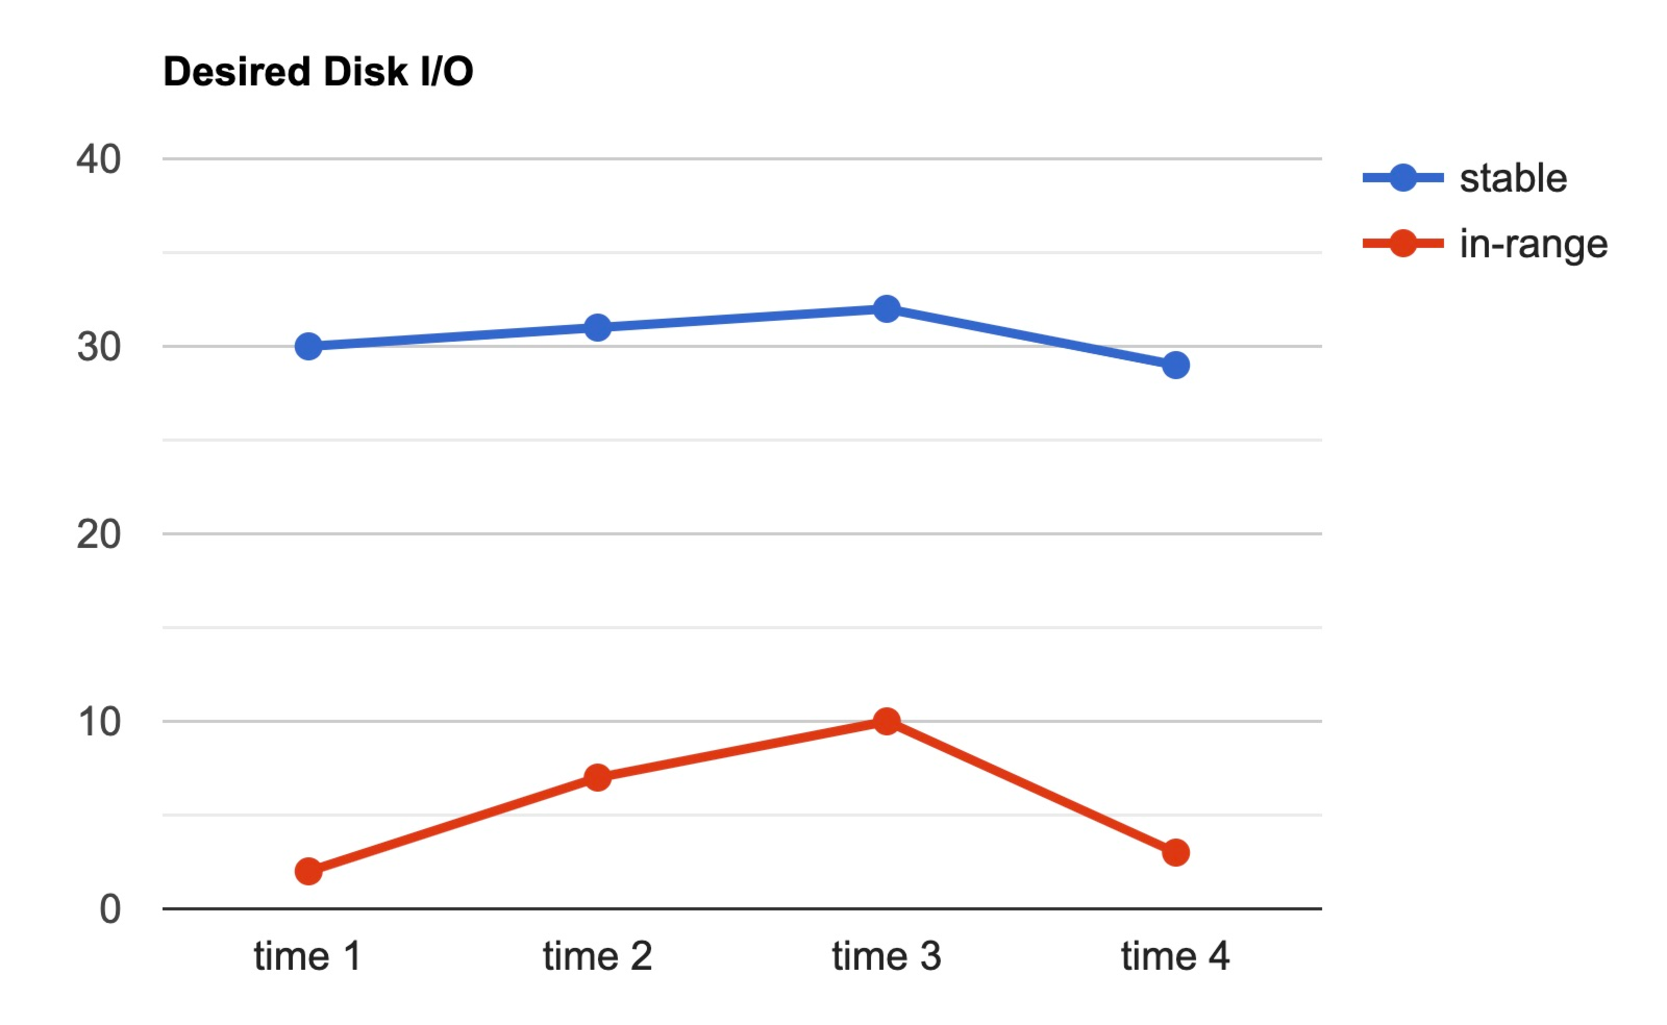
\includegraphics[width=\linewidth]{resources/desired.pdf}
    \caption{desired disk I/O util pattern}
    \label{fig:desired}
  \end{figure}

  \begin{figure}
    \centering
      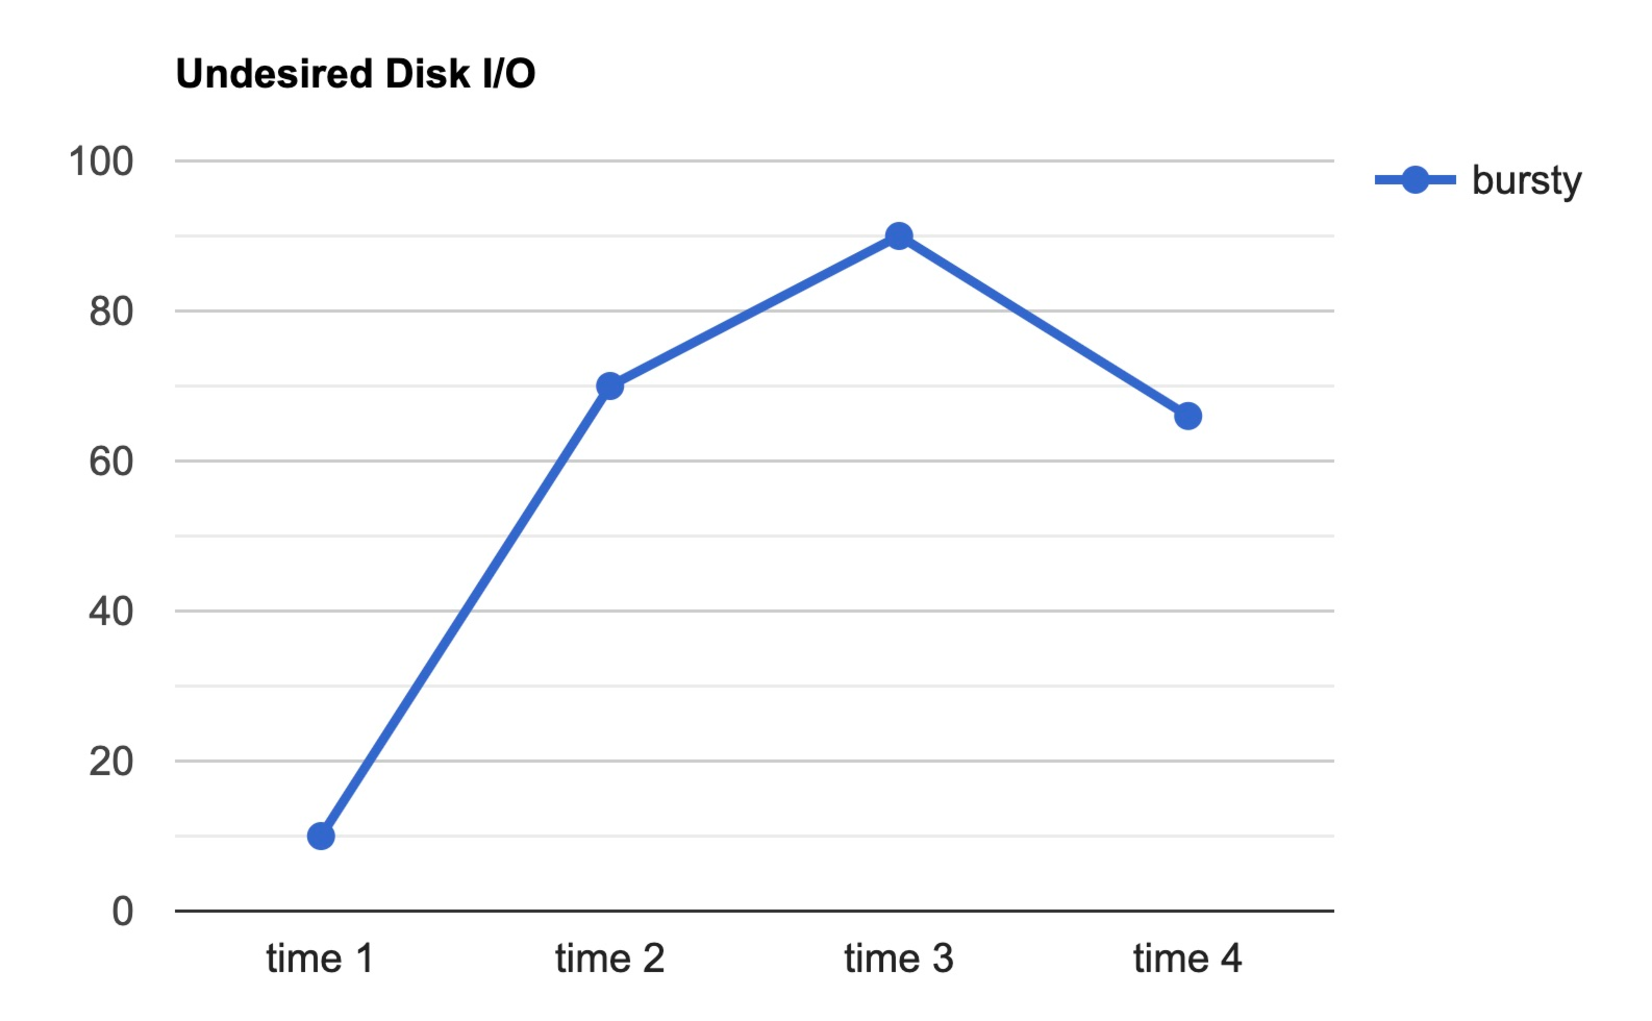
\includegraphics[width=\linewidth]{resources/undesired.pdf}
      \caption{undesired disk I/O util pattern}
      \label{fig:undesired}
    \end{figure}
Can we also take the approach that set a target disk throughput for containers, just as what was done to applications in Maestro? Unfortunately, we can not do the same things with containers, since applications running inside the containers are completely transparent to us. We are not able to know their feature, types, and behavior. We can't even know how many applications would be running in a single container, and how is the target going to fluctuate as the number of containers changes.\\

However, there are still some intuitions that might help with the problem: can we predict the immediately coming disk utilization of a container based on its disk utilization data points in the past period? After a thorough retrospect of the experiences we had with cloud services, we think the answer is yes. In industry, the containers that share a single host machine with others are not supposed to have an unstable and harsh disk utilization pattern. As time goes on, their utilization curves should either remain inside a very stable range, or show some fluctuation at a general low usage level \ref*{fig:desired}. Only under this assumption, these containers can coexist on a single node. For those containers whose guest applications have demanding requirement for disk, such as frequent bursty I/O and high disk utilization \ref*{fig:undesired}, we assert that it's better not to deploy them on a shared machine with any other containers, since it won't be fair for other stake holders. \\

We introduce 2 notion here. The first one is \textbf{lifeline}. If a container shows a stable disk utilization in the past time period, it’s very likely that it needs at least this amount of utilization in order to serve its duty faithfully. We refer this amount of utilization as the lifeline of the container. The second one is abruption. If a container is showing a burst in its I/O utilization, it's very likely due to some abnormal/malicious events. e.g., image downloading, DoS attack. We refer this kind of traffic pattern as abruption. To summarize, we hold the view that lifeline deserves higher priority than abruption! \\

So for those containers with stable disk utilization pattern, we can gather  their historic data points, and then do some aggregation to estimate their lifelines. The aggregation is not necessarily supposed to be sophisticated. Simple and straightforward operatio, such as average, should be able to serve as a good-enough lifeline estimation. \\

On top of the estimated lifelines, we can experiment and apply various isolation policy. For the firstly isolation policy in this initial version of Aridac, we introduce an elastic ratio \textit{P}. We assert the next-round utilization will be in the range of up to \textit{lifeline*(1+P)}. And this is value, \textit{lifeline*(1+P)}, will be set as the cap of disk utilization in the coming round for a container.\\

\section{Design \& Implementation}
\begin{figure}
  \centering
    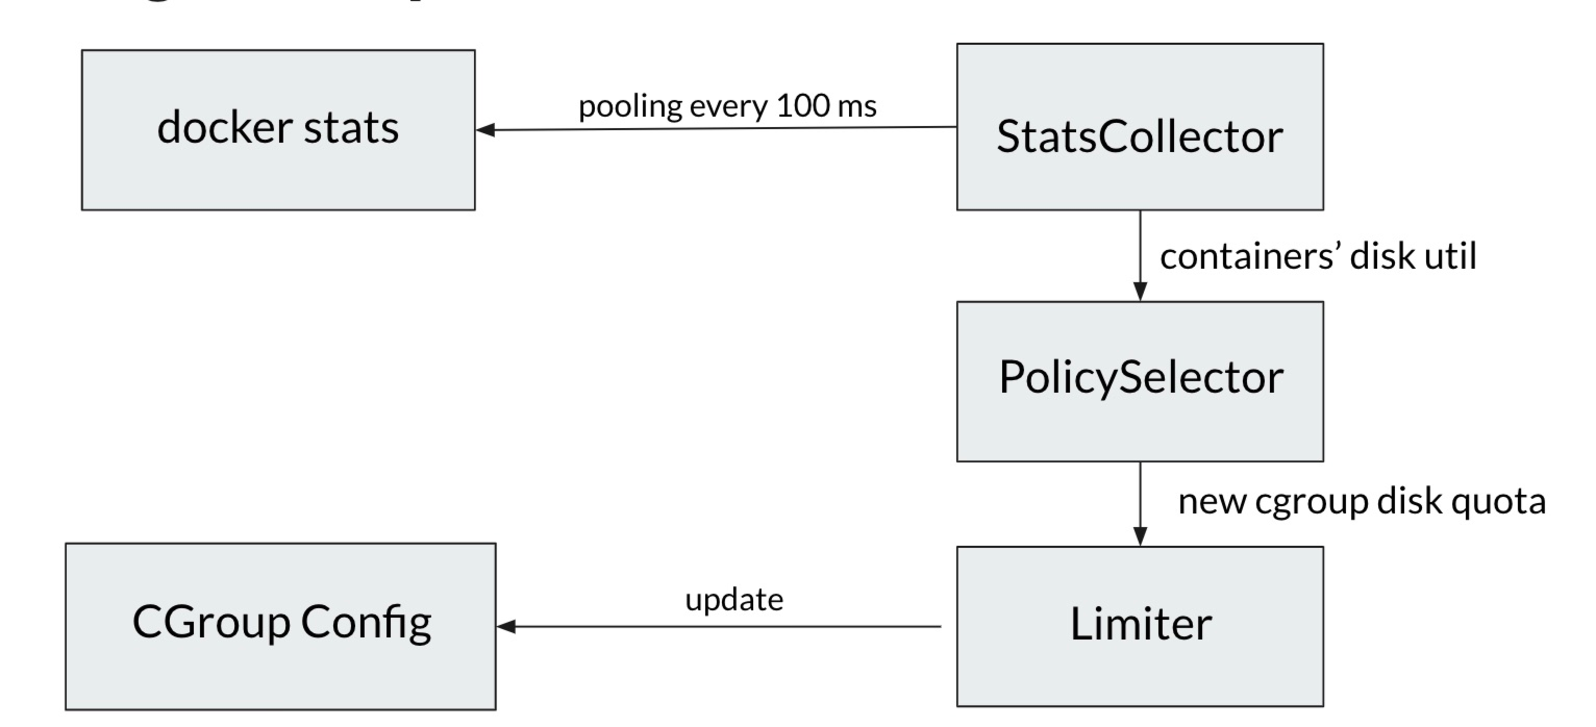
\includegraphics[width=\linewidth]{resources/design.pdf}
    \caption{system overview}
    \label{fig:design}
  \end{figure}
We present the design \ref{fig:design} and implementation overview of Aridac in the coming paragraphs. \\

\subsection{Stats Collector}
The architecture of Aridac is pipelined. First, Aridac depends on the Docker native stats command \textit{docker stats} in order to get the disk throughput of container. The disk throughout shown by docker stats is the accumulative disk throughout since the start of a container. So we subtract the previous throughput on the latest one to get the delta value. And this delta value is the amount of disk throughput that's been done between the last 2 sampling points. Since the interval of the refreshing of the output stream of docker stats is somewhat varying, the StatsCollector of Aridac will keep polling the output stream of docker stats command at a fixed interval that is a lot smaller than the one of the output stream in order to process the latest data in a timely manner. The StatsCollector also record the timestamp of its last receiving refresh from the output stream, so that we can calculate the disk throughput per unit time. And disk throughput per unit time will be used to calculate the disk utilization rate of a container.At the end of StatCollector, we get the disk utilization rate of every living container. We will push the rate to a bounded queue with a fixed length of N. This queue is the output of StatsCollector and also the input PolicySelector.\\

\subsection{Policy Selector}
Once the execution enters PolicySelector, we then do various aggregation to the collected data and select the isolation policy we want to apply. In the initial version, we implemented the simple aggregation that takes the average of all these history utilization rates inside the bounded queue. And the average value we get is the lifeline. And the policy we use is to set a cap disk utilization value \textit{lifeline*(1+P)} for each individual container.The current implementation the \textit{P} we use is 20\%. \\

And after having all the caps calculated, we check if the sum of the cap is bigger than 1. If so, it shows the disk contention is pretty intense and the system enters a unstable state, where disk utlization may quickly reach 100\% and the performance of guest applications could be severely jeopardized. So in this case, we will prompt alert to the user or system admin just so to let them be aware of the resource shortage, so that they can take measures like redeploying some containers in another machine, or add more disks to ease th situation. An interesting improvement we can do here, is to implement an auto disk scaling mechanism. With the help of an auto tool, the redeployment and scaling of the disk can be triggered without the intervention of any human resource. And the tool can also be more responsive to problems than human can be.\\


\subsection{Limiter}
Limiter is the abstraction of Linux cgroup resource control mechanism. There are several interfaces provided in the limiter, which are used to set the cap of disk input and disk output rate for any specific process. In the PolicySelector, after we have calculated the caps, we then call the interface in limiter to actually send the command to the system, by writing our new caps into the config file of each individual cgroup. For docker containers, each one of them has its own cgroup, whose config file can be indexed with the container id. So it's very convenient for us to set the caps in Limiter.

\section{Evaluation}

In this section, we aim to prove two major things. First, the scenario of resource preemption exist; second, to test if our policy is able to prevent the resource preemption.
and the quota limit can adapt the dynamic desire of application (e.g. increase or decrease).

\subsection{Workload Design}

\begin{itemize}
  \item \textbf{Workload 1} Two containers A and B running with same rate (200KiB/s) in the beginning. At some point, B's I/O usage goes high without limit (2MiB/s), preempting A's resource.
  \item \textbf{Workload 2} Two containers A and B running with same rate (200KiB/s) in the beginning. At some point, B's I/O usage goes high without limit (2MiB/s), preempting A's resource. After a while, B's usage goes back to normal rate (200KiB/s).
\end{itemize}

Our policy should prevent the above resource preemption. Also, the quota allocated by our policy should keep align with the containers' desire dynamically. The only difference between two workloads is that, in workload 2, B's usage goes back to its normal rate, where our policy should be able to adjust the quota low. \\


% conference papers do not normally have an appendix

\section{Conclusion}
We conducted a thorough investigation about the problems existed for disk contention under modern containerized environment. We found out that the disk resource isolation level among containers is not good enough to ensure a consisten behavior pattern and perfornmance of the whole system. On a shared physical node where multiple containers are running stably, disk contention \& preemption may occur due to unexpected events.\\

We further did our literature review in search of disk utilization quota control relevant topics. And the work we found served as good insights, but cannot be directly applied to our problem because of the difference in domain. \\

We figured out the historic disk utilization statistics may be useful in predicting the incoming short-term disk utilization. And we followed this hypothesis and implemented Aridac, with a pipelined system architecture which includes 3 phases namely StatsCollector, PolicySelector, and Limiter. We futher show that Aridac achieved the desired adaptive disk resource isolation capability under the simulated environment with several carefully-designed workloads.\\

To conclude, with Aridac, we are able to adjust the resource cap for each container adaptively, so that programs in the guest containers could maintain a consistent performence throughout their lifetime.

\section{Problems Encountered}
We encountered many troubles throughout the whole journey. For example, we were disturbed by not being able to reproduce the case where a container with high disk I/O could preempt the disk share of the other container. Also, at the beginning stage of the evaluation, we planned to use Death Star microservice benchmark as the testbed. But later we found that the launching of Death Start will cause a lot of dependency issues and mess up the test environment. And the other time-consuming task is to find the suitable disk I/O generator. We tried different kinds of approach, from self-improvised C program, to the dd shell command, and finally the fio. And the usage of fio is a bit complex, with a lot of available arguments and options. Fortunately the documentation is very helpful, and we were able to find everything we want from it.\\

\section{Future Work}

% In our final paper, we will first introduce the resource isolation problem of the container environment and discuss the background and related work. Next, we will briefly outline the system design and implementation of Aridac. Last, we will describe our experimental setup, including what machines and environments were used, what workload we developed to test our implementation. The most crucial part of the paper will be concerned with describing and evaluating our methods for container resource isolation. We will provide performance analyses, and conclude with a discussion about potential optimization schemes, and if possible, a set of benchmarks for more detailed performance evaluation.\\

% The early stage of our project will be analyzing existing issues caused by weak isolation of the container environment, researching existing relative works on different levels of virtualization technologies and container resource isolation, and finding out a doable logic for performing a dynamic resource isolation scheme in the container environment. Our project will then focus on developing a dynamic resource isolation policy for the container environment, to achieve the goal of balancing the resources among multiple containers running on the same physical machine. We will implement a program working on dynamic resource allocation and isolation for containers sharing the same underly resources, and may try out different policies for resource allocation of network bandwidth and disk I/O of the physical machine to learn their performance characteristics.\\

% We will design and develop a set of workloads to simulate some most common applications running in the industry. Then we will let a few containers run that workload and monitor their resource and performance, to see if any rapid resource obtaining will happen and broke the resource allocation balancing. If we can reproduce the scenario of container resource exhausting caused by weak isolation, then we may follow up by testing whether it strengthens the resource isolation among containers and result in better overall performance.\\

% To measure the success of our project, we will focus on completeness rather than performance. But we will examine if there are any possible optimization for the implementation and leave it as potential future works. Other possible topics include comparisons between static isolation approaches and our dynamic isolation approach, discussing the pros and cons of using different levels of encapsulations and virtualization technologies, and even recursive virtualization for more stable overall performance. We will also try to figure out the weight of different resources in the container environment, discussing trade-offs and complexities. Hopefully, the results and discussions will help us know the effectiveness and generality of the dynamic isolation approach for various working scenarios.\\

% Here are some questions that our experiments will answer:

% • What kinds of scenarios will require strong resource isolation for applications running in the container environment?

% • Is dynamic resource allocation and isolation beneficial for the overall performance of applications running in the container environment?

% • What are the appropriate resource allocation approaches for applications with different characteristics?

% • How strong is the isolation provided by the dynamic isolation and allocation approach? 

% • How stabilized has the performance of the container environment been achieved after adopting stronger isolation?

% • What is the overall overhead of our approach? 

% By the date this interim report was written, we have made some achievement in the aspects that are mentioned in section 4.1-4.3. Below is a tentative schedule for the future work.\\

% \begin{itemize}
%   \item By 15th April, we plan to achieve the 75\% goal. We will finish the 3 essential components of Aridac, which are the load generation module, the runtime machine metrics monitor module, and the dynamic resource isolation module. And we will make sure that Aridac achieves a better performance in a several given typical tests.
%   \item By 30th April, we plan to achieve the 100\% goal, which seeks to build a comprehensive collection of typical workloads under containerized environment. And Aridac will excel in all of those tests, with concrete benchmark given in the report. 
% \end{itemize}





% trigger a \newpage just before the given reference
% number - used to balance the columns on the last page
% adjust value as needed - may need to be readjusted if
% the document is modified later
%\IEEEtriggeratref{8}
% The "triggered" command can be changed if desired:
%\IEEEtriggercmd{\enlargethispage{-5in}}

% references section

% can use a bibliography generated by BibTeX as a .bbl file
% BibTeX documentation can be easily obtained at:
% http://mirror.ctan.org/biblio/bibtex/contrib/doc/
% The IEEEtran BibTeX style support page is at:
% http://www.michaelshell.org/tex/ieeetran/bibtex/
%\bibliographystyle{IEEEtran}
% argument is your BibTeX string definitions and bibliography database(s)
%\bibliography{IEEEabrv,../bib/paper}
%
% <OR> manually copy in the resultant .bbl file
% set second argument of \begin to the number of references
% (used to reserve space for the reference number labels box)
\bibliographystyle{IEEEtran}
\bibliography{bibi}




% that's all folks
\end{document}